\documentclass[crop,tikz]{standalone}
\usetikzlibrary{backgrounds}
\colorlet{blue}{cyan}
\tikzset{
  inverted/.style = {
    color=white,
    background rectangle/.style={fill},
    show background rectangle
  }
}

\usepackage{pgfplots}
\tikzset{>=latex}
\colorlet{green}{green}

\pgfplotsset{
  inverted/.style = {
    every axis legend/.append style={
      draw=white,
      fill=black,
      text=white
    }
  },
  every non boxed x axis/.append style={
    axis line style={-latex}
  },
  every non boxed y axis/.append style={
    axis line style={-latex}
  }
}

\begin{document}
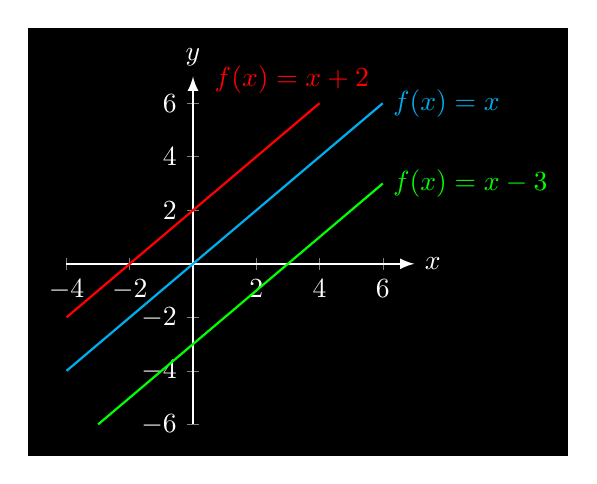
\begin{tikzpicture}[inverted,inverted]
\begin{axis}[inverted,
  thick,
  width=6cm,
  height=6cm,
  xlabel={$x$},
  ylabel={$y$},
  xmin = -4, xmax = 7,
  ymin = -6, ymax = 7,
  axis y line=middle,
  axis x line=middle,
  xlabel style={at=(current axis.right of origin), anchor=west},
  ylabel style={at=(current axis.above origin), anchor=south},
  xtick distance=2,
  ytick distance=2,
  samples=10,
  smooth,
  clip=false,
  ]
  \addplot[red, domain=-4:4] {x+2} node[above,xshift=-1em] {$f(x)=x+2$};
  \addplot[blue, domain=-4:6] {x} node[right] {$f(x)=x$};
  \addplot[green, domain=-3:6] {x-3} node[right] {$f(x)=x-3$};
\end{axis}
\end{tikzpicture}
\end{document}
